% ncse_new/p1_SystemsOfEquations/ch1_MatVec/ex_ArrowMatrixVector.tex
% the exercise requires:    arrowmatvec.m    arrowmatvectiming.eps    arrowmatvectiming.jpg
% the solutions require:    arrowmatvec2.m    arrowmatvec2timing.m    arrowmatvec2timing.eps

\begin{samproblem}{prb:ArrowMatrixVector}{Arrow matrix-vector multiplication (core problem)}{
Consider the multiplication of the two ``arrow matrices'' $\VA$ with a vector $\Vx$,
implemented as a function \texttt{arrowmatvec(d,a,x,y)} in \cref{cpp:arrowmatvec}
}
\begin{samcode}[C++-code]{cpp:arrowmatvec}{multiplying a vector with the product of two ``arrow matrices''}
  \lstinputlisting[style=cpp]{Chapters/MatrixVector/CPP/arrowmatvec.hpp}
\end{samcode}

\begin{samhint}
This \cpp~ code is provided as file \texttt{arrowmatvec.hpp}.
\end{samhint}

%%%%%%%%%%%% SUBPROBLEM 1

\begin{subproblem}{sp:1}[1]
  For general vectors $d = (d_1, \dots, d_n)^\top$ and $a = (a_1, \dots, a_n)^\top$, sketch the matrix $\VA$ created in \autoref{cpp:arrowmatvec}.

  % BEGIN ================ SOLUTION  ================   %
  \begin{samwriteprbpart}{solfile}
    \begin{writeverbatim}{prbfile}
      \begin{samsolution}
        $\VA=\begin{pmatrix}
         d_1 &     &        &         &  a_1     \\
             & d_2 &        &         &  a_2     \\
             &     & \ddots &         &  \vdots  \\
             &     &        & d_{n-1} &  a_{n-1} \\
         a_1 & a_2 & \dots  & a_{n-1} &  d_n     \\
        \end{pmatrix}$
      \end{samsolution}
    \end{writeverbatim}
  \end{samwriteprbpart}
  % END ================== SOLUTION  ================   %
\end{subproblem}

%%%%%%%%%%%% SUBPROBLEM 2

\begin{subproblem}{sp:2}[2]
  The timing results for \texttt{arrowmatvec.cpp} are available in \autoref{fig:arrowmatvectiming}. 
  Give a detailed explanation of the results.

  \begin{figure}[ht]
    \centering
    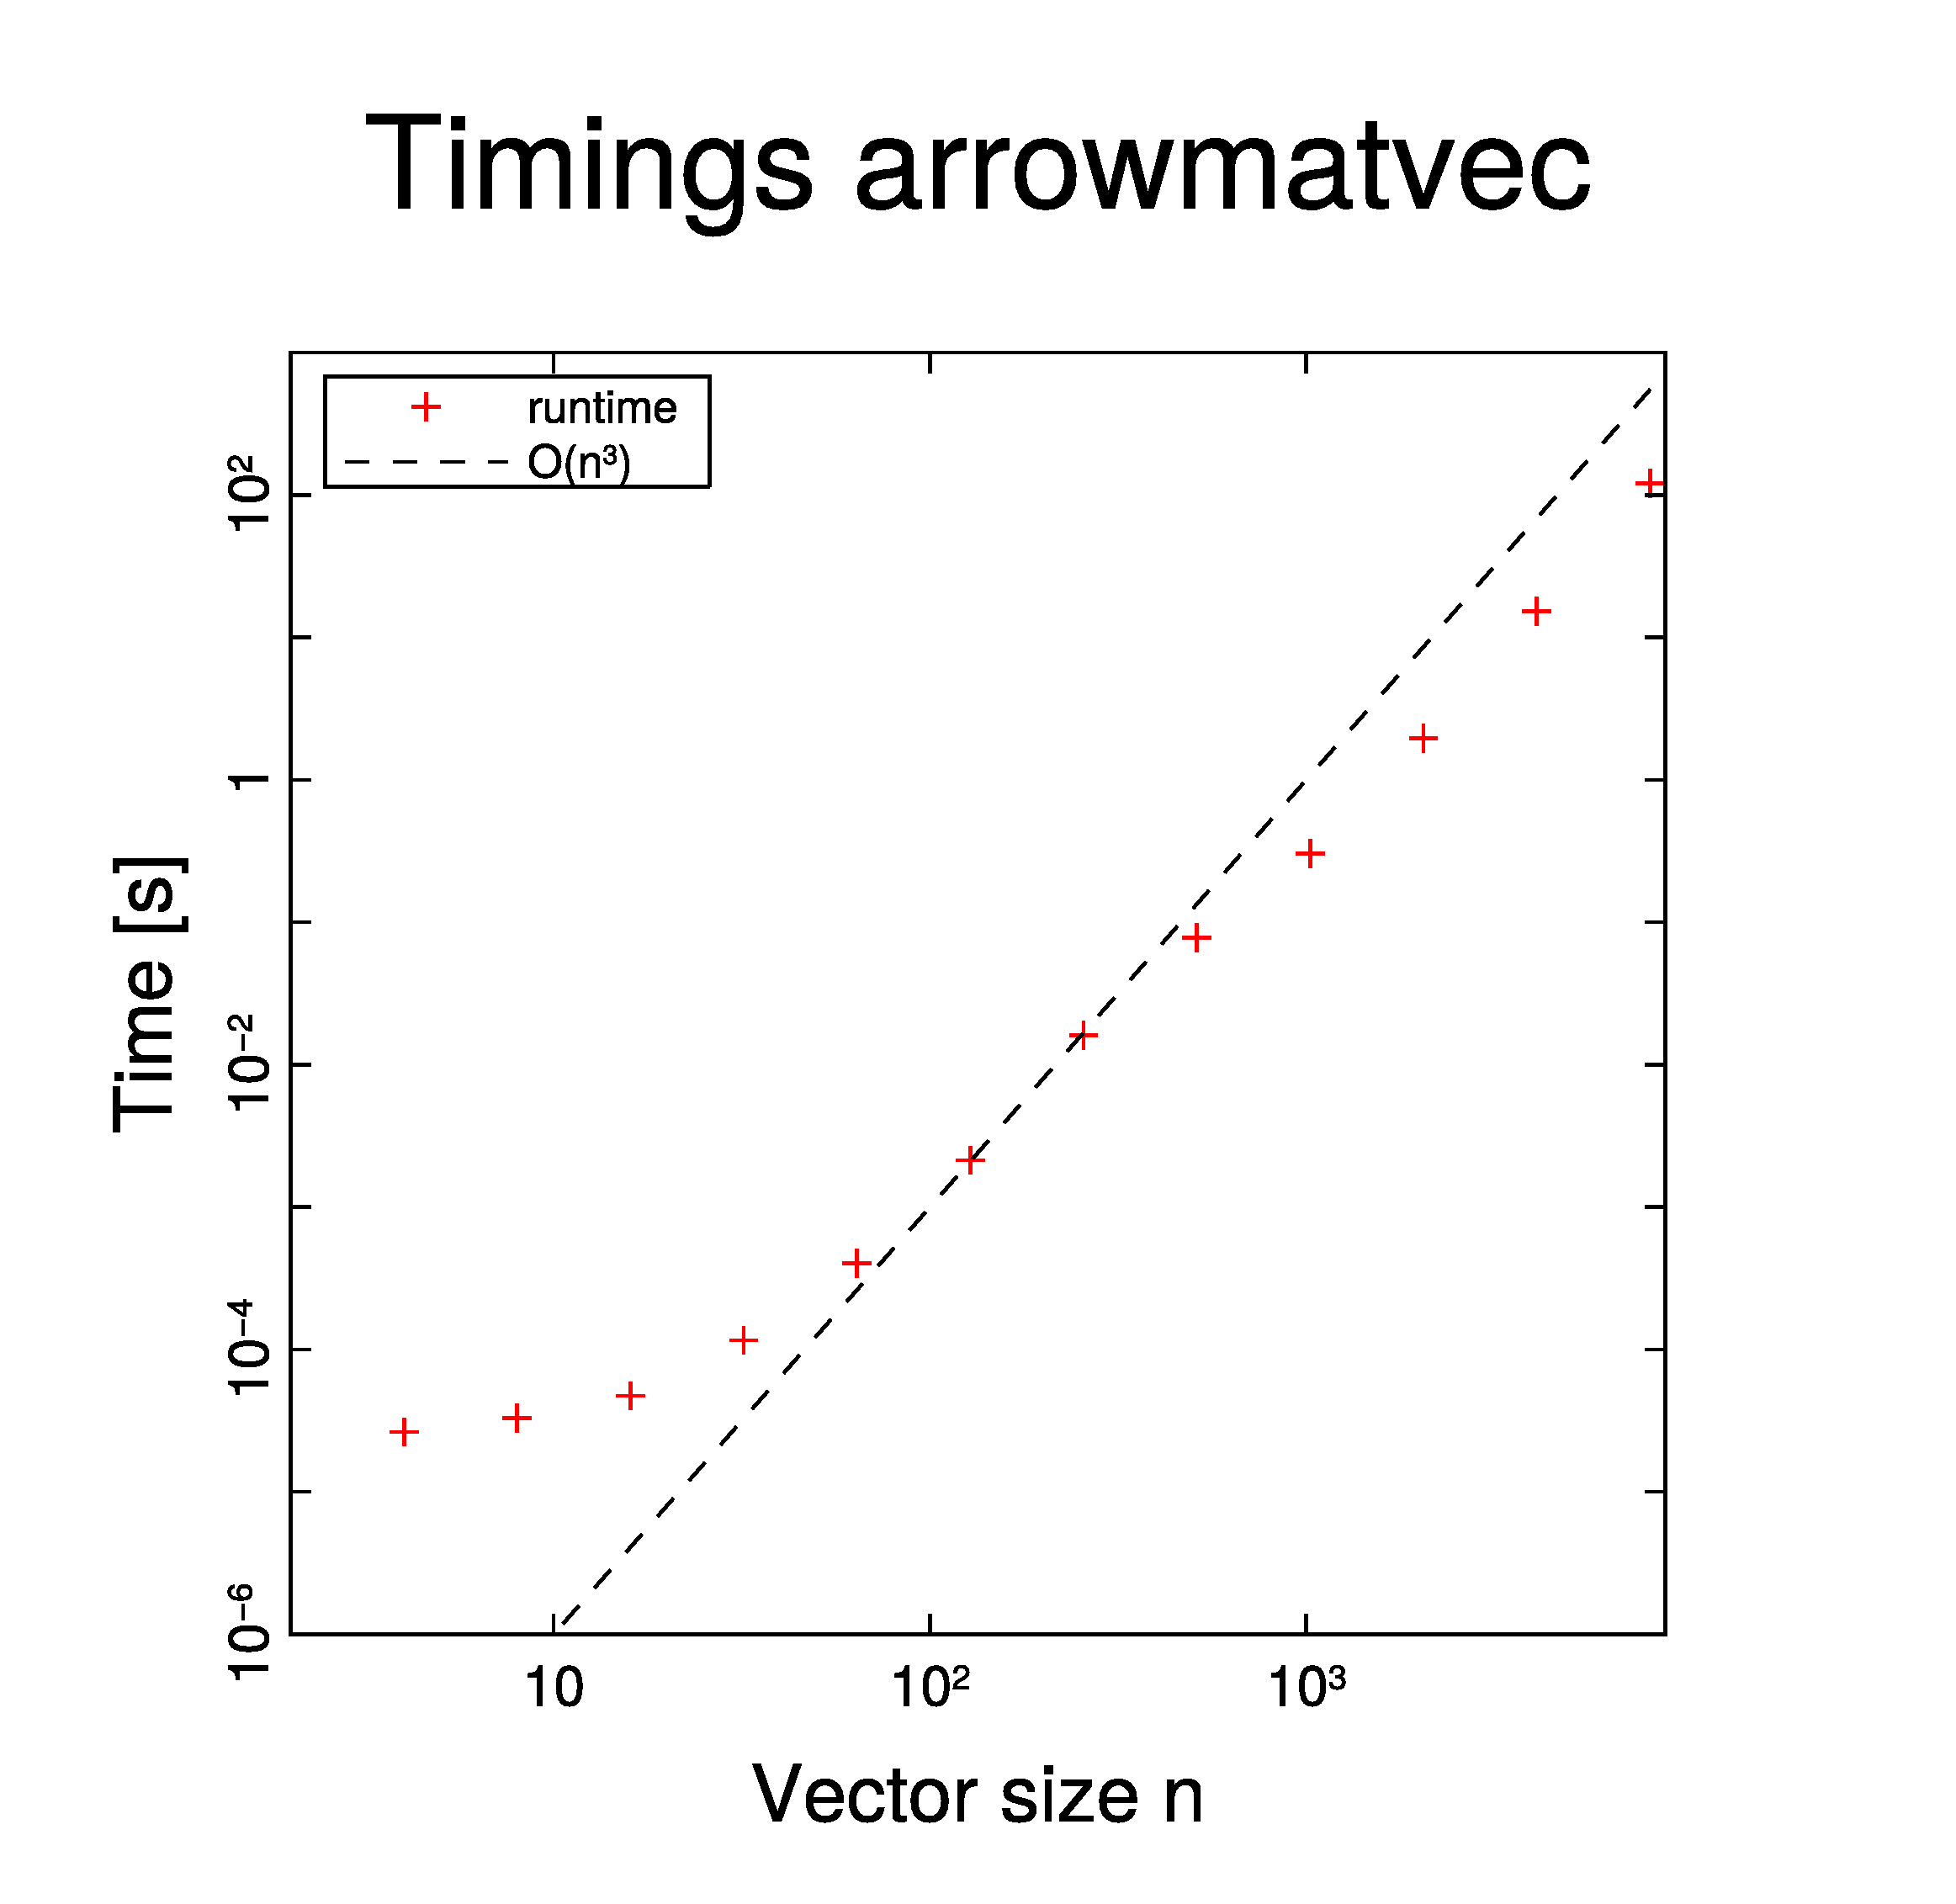
\includegraphics[width=0.8\textwidth]{Chapters/MatrixVector/PICTURES/arrowmatvectiming.eps}
    \caption{timings for \texttt{arrowmatvec(d,a,x)}}
    \label{fig:arrowmatvectiming}
  \end{figure}

  \begin{hint}
    This \cpp~ created figure is provided as file
    \texttt{arrowmatvectiming.\{eps,jpg\}}.
  \end{hint}

  % BEGIN ================ SOLUTION  ================   %
  \begin{samwriteprbpart}{solfile}
    \begin{writeverbatim}{prbfile}
      \begin{samsolution}
      The standard matrix-matrix multiplication has runtimes growing with $O(n^3)$ 
      and the standard matrix-vector multiplication has runtimes growing with $O(n^2)$. 
      Hence, the overall computational complexity is dominated by $O(n^3)$.
      \end{samsolution}
    \end{writeverbatim}
  \end{samwriteprbpart}
  % END ================== SOLUTION  ================   %
\end{subproblem}

%%%%%%%%%%%% SUBPROBLEM 3
\begin{subproblem}{sp:3}[3]
  Write an \emph{efficient} \cpp~ function 
  \begin{samcode}[C++-code]{cpp:sp3}{Function prototype}
    \begin{lstlisting}[style=cpp]
template <class Matrix>
void arrowmatvec2(const Matrix& d, const Matrix& a, const Matrix& x, Matrix& y)
    \end{lstlisting}
  \end{samcode}
  that computes the same multiplication as in code \ref{cpp:arrowmatvec} but with optimal asymptotic complexity with respect to {$n$}.
  Here \texttt{d} passes the vector $(d_{1},\ldots,d_{n})^{T}$ and \texttt{a} passes the vector $(a_{1},\ldots,a_{n})^{T}$.

  % BEGIN ================ SOLUTION  ================   %
  \begin{samwriteprbpart}{solfile}
    \begin{writeverbatim}{prbfile}
      \begin{samsolution}
      Due to the sparsity and special structure of the matrix, it is possible to write a more efficient implementation than the standard matrix-vector multiplication. 
      See code listing \ref{cpp:arrowmatvec2}

      \begin{samcode}[C++-code]{cpp:arrowmatvec2}{implementation of the function \texttt{arrowmatvec2}}
        \lstinputlisting[style=cpp]
        {Chapters/MatrixVector/CPP/arrowmatvec2.hpp}
      \end{samcode}

      \end{samsolution}
    \end{writeverbatim}
  \end{samwriteprbpart}
  % END ================== SOLUTION  ================   %

\end{subproblem}
%%%%%%%%%%%% SUBPROBLEM 4

\begin{subproblem}{sp:4}[1]
  What is the complexity of your algorithm from sub-problem \ref{sp:3} (with respect to problem size $n$)? 

  % BEGIN ================ SOLUTION  ================   %
  \begin{samwriteprbpart}{solfile}
    \begin{writeverbatim}{prbfile}
      \begin{samsolution}
      The efficient implementation only needs two vector-vector element-wise multiplications and one vector-scalar multiplication. 
      Therefore the complexity is $O(n)$.
      \end{samsolution}
    \end{writeverbatim}
  \end{samwriteprbpart}
  % END ================== SOLUTION  ================   %

\end{subproblem}

%%%%%%%%%%%% SUBPROBLEM 5

\begin{subproblem}{sp:5}[2]
  Compare the runtime of your implementation and the implementation given in code \ref{cpp:arrowmatvec} for $n=2^{5,6,\ldots,12}$.
  Use the \texttt{std::chrono} package (see \hyperlink{link}{\Blue{here}}) or use the provided library \texttt{timer.h}.

  % BEGIN ================ SOLUTION  ================   %
  \begin{samwriteprbpart}{solfile}
    \begin{writeverbatim}{prbfile}
      \begin{samsolution}
      The standard matrix multiplication has runtimes growing with $O(n^3)$.
      The runtimes of the more efficient implementation are growing with $O(n)$.
      See \autoref{cpp:arrowmatvec2timing} and Figure~\ref{fig:arrowmatvec2timing}.

      \begin{samcode}[C++-code]{cpp:arrowmatvec2timing}{Execution and timings of \texttt{arrowmatvec} and \texttt{arrowmatvec2}}
        \lstinputlisting[style=cpp]
        {Chapters/MatrixVector/CPP/arrowmatvec2timing.cpp}
      \end{samcode}

      \begin{figure}[ht]
        \centering
        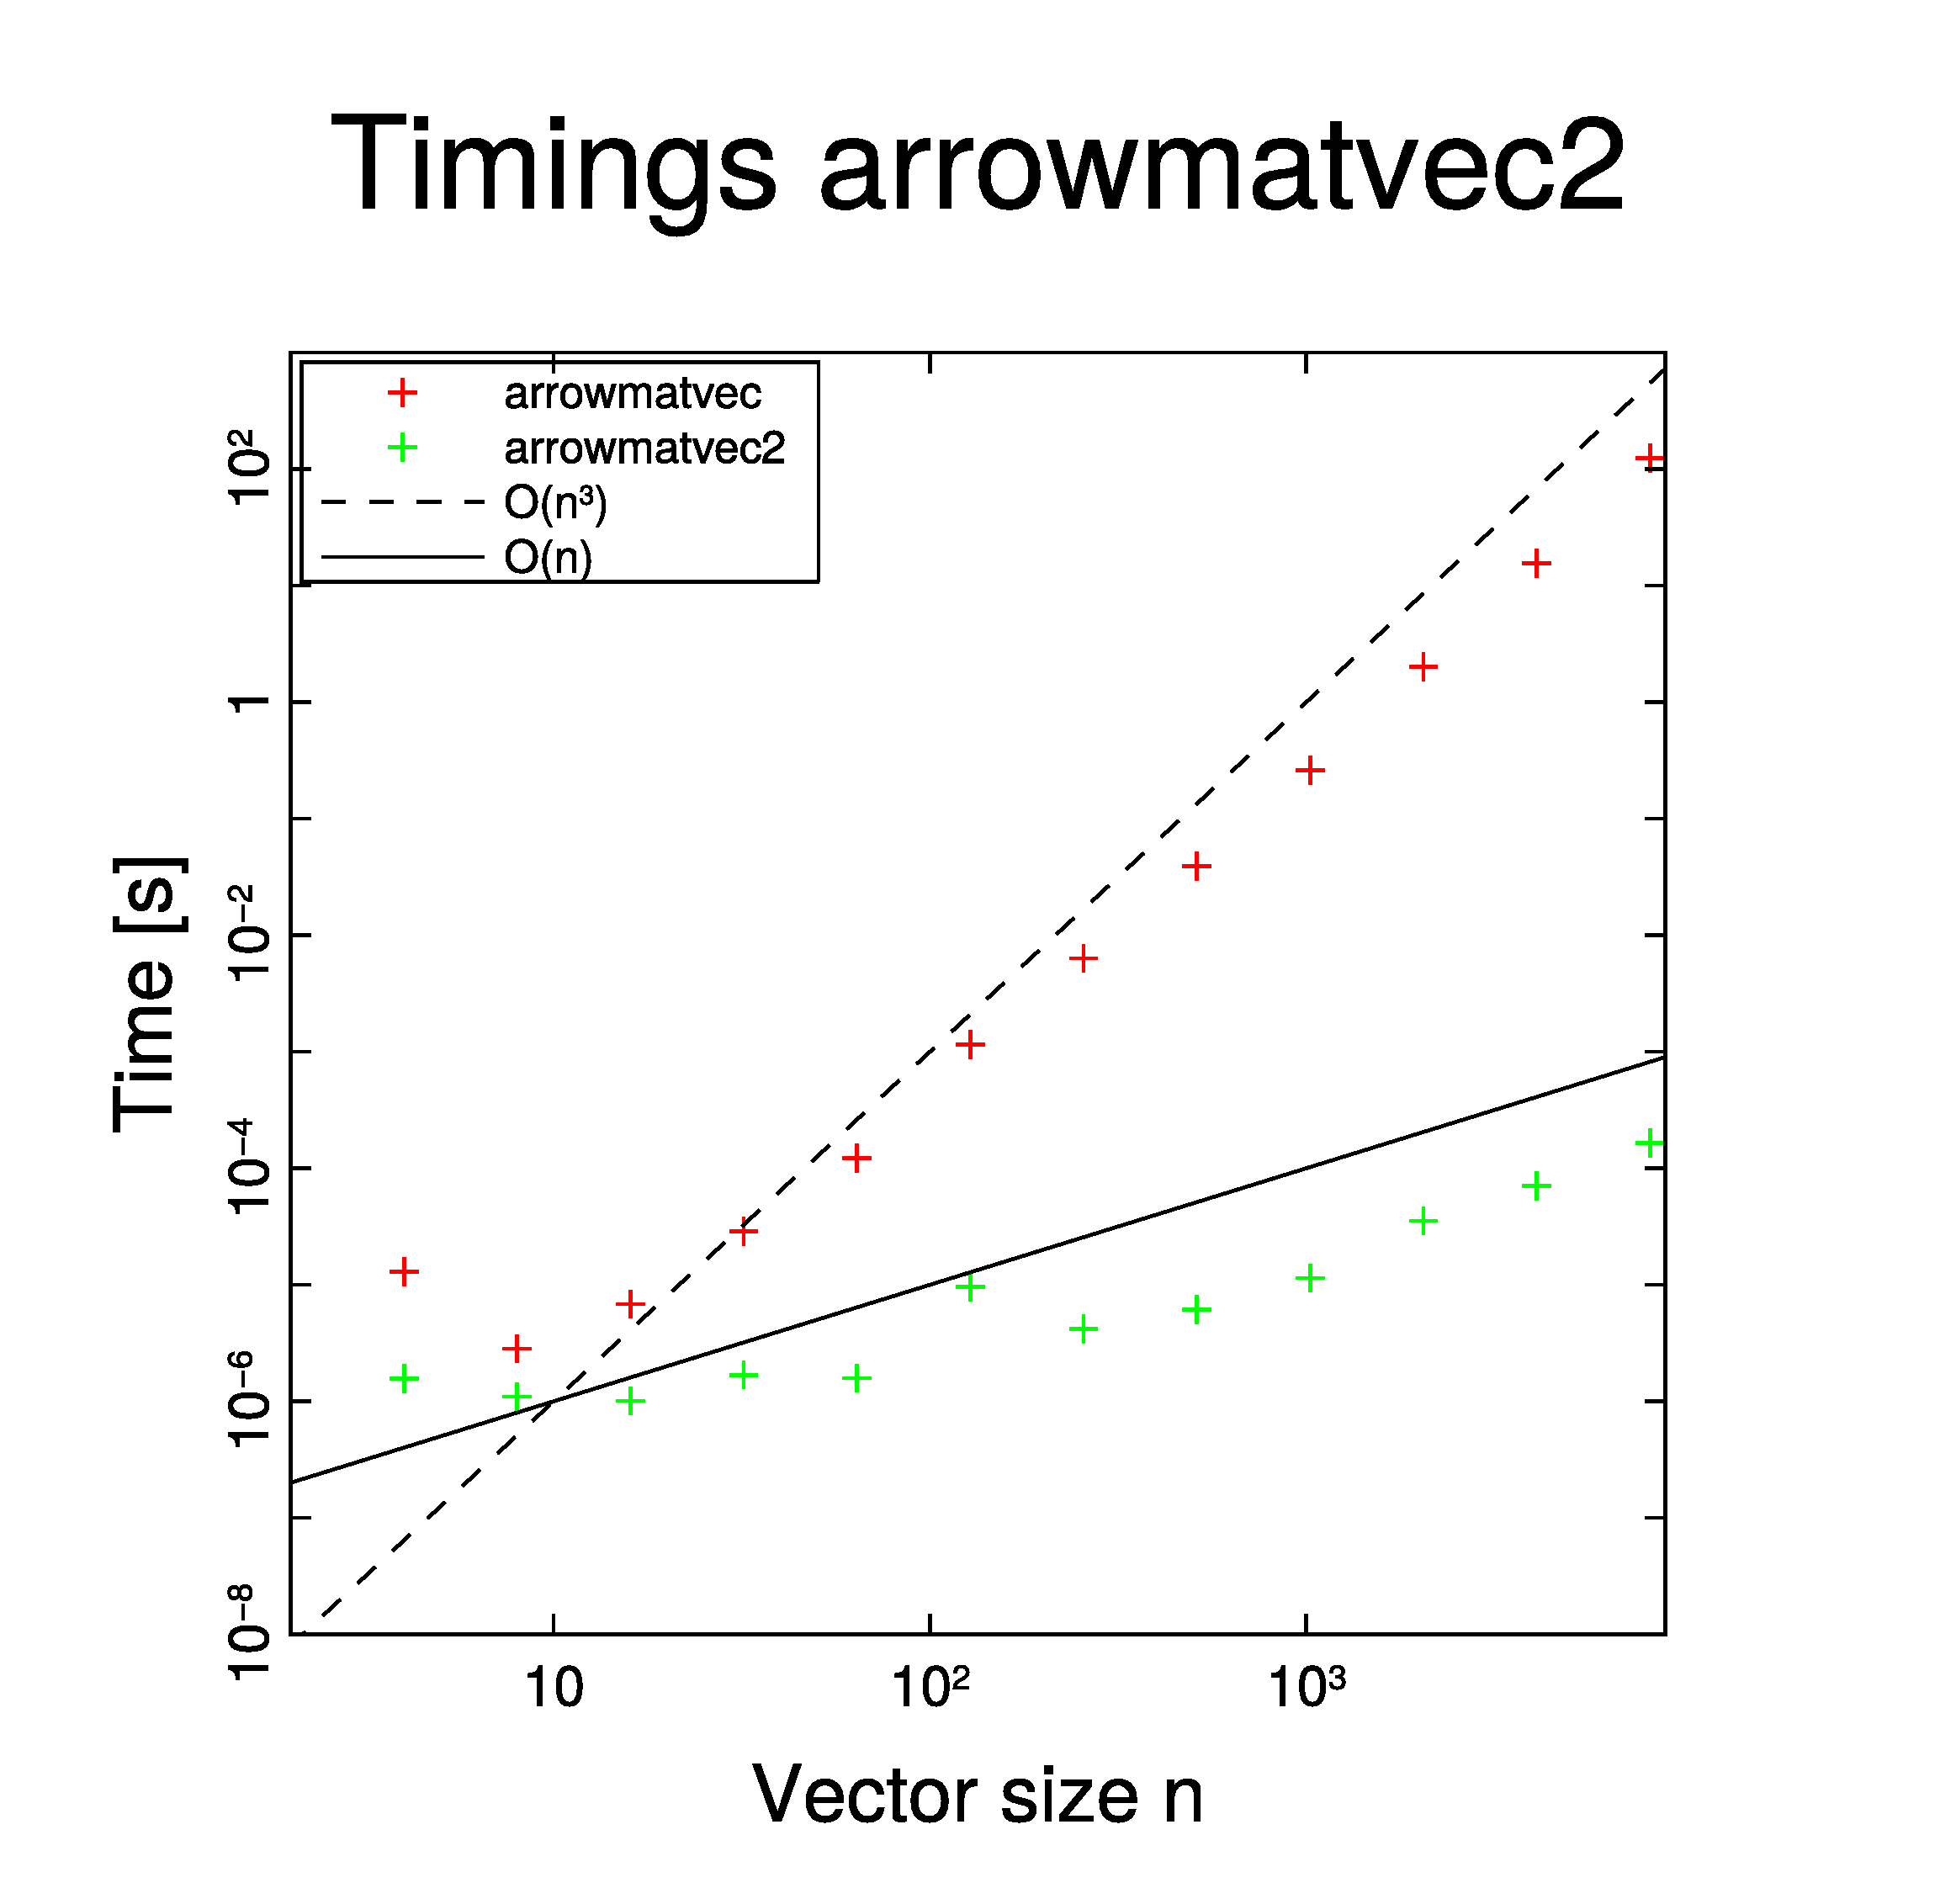
\includegraphics[width=0.8\textwidth]{Chapters/MatrixVector/PICTURES/arrowmatvec2timing.eps}
        \caption{timings for \texttt{arrowmatvec2(d,a,x,y)}} \label{fig:arrowmatvec2timing}
      \end{figure}
      \end{samsolution}
    \end{writeverbatim}
  \end{samwriteprbpart}
  % END ================== SOLUTION  ================   %

\end{subproblem}


%% this subproblem does only make sense if the other problems are using Matlab codes
%\begin{subproblem}[1] \label{subprb:ArrowMatrixVector_6}
%Write the \eigen{} codes corresponding to the functions \texttt{arrowmatvec} and \texttt{arrowmatvec2}.
%
%\begin{solution}
%See Listing~\ref{cppc:arrowmatvec} and Listing~\ref{cppc:arrowmatvec2}.
%
%\lstinputlisting[style=cpp,caption={Implementation of \texttt{arrowmatvec}  in \eigen{}},label={cppc:arrowmatvec}]
%{\problems/\chpt/CPP/arrowmatvec.cpp}
%
%\lstinputlisting[style=cpp,caption={Implementation of \texttt{arrowmatvec2}  in \eigen{}},label={cppc:arrowmatvec2}]
%{\problems/\chpt/CPP/arrowmatvec2.cpp}
%\end{solution}
%\end{subproblem}

\end{samproblem}
